\chapter{结论与展望}
\label{cha:conclusion}

\section{主要结论}
\label{sec:conclusion}
为了充分发挥先进绝热压缩空气储能这一颇具吸引力的储能理念对电力系统实现可持续的高比例可再生能源电量渗透目标的支撑作用,本文通过挖掘其具有的常规灵活性(能量搬移与容量备用)、供能灵活性(热电联供与热电联储)及接口灵活性(机械输入与机械输出),从网侧、荷侧及源侧分别研究了先进绝热压缩空气储能电站、先进绝热压缩空气能量枢纽及内嵌先进绝热压缩空气储能的灵活风机的设计建模、调度运行及市场运营等问题。特别地,结合先进绝热压缩空气储能在可再生能源系统运行中需要实现的外部系统级宽工况运行条件对内部组件级部分负载特性的影响,研究了计及宽工况特性的热力学仿真模型。本文的主要成果和创新点可以归纳为以下四点:

\textbf{(1)在热力学特性建模方面,提出了计及组件部分负载特性的先进绝热压缩空气储能通用稳态热力学仿真模型,并分析了典型系统的典型运行及供能模式。}

计及定压-定压、定压-滑压、滑压-定压、滑压-滑压等典型压缩膨胀运行模式(压力视角),提出了基于热力学第一定律与热力学第二定律的仅电能供应与热电多能联供(温度视角)的稳态热力学仿真模型。基于建立的热力学仿真模型分析了一典型AA-CAES系统在典型运行模式及供能模式下的内部热力学特性及外部供能特性,为网侧储能电站、荷侧能量枢纽及源侧灵活风机等三种场景下对应先进绝热压缩空气储能应用形式的建模分析、调度运行及市场运营的研究奠定基础。

\textbf{(2)在挖掘常规灵活性方面,提出了刻画先进绝热压缩空气储能内部多能流耦合及宽工况运行特性的储气储热双SOC模型及其扩展形式,调度与运营方法。}

基于热力学稳态仿真模型与特性曲线,提出了刻画不同于常规电池储能的独特的内部压力势能与压缩热能多能流耦合热力学特性的四条热力学特性曲线。基于热力学特性曲线,构建了先进绝热压缩空气储能宽工况储气-储热双SOC 能量模型、能量与备用模型及其扩展模型。将双SOC模型应用于风-储协同系统发电能力评估、市场策略竞标等问题,指导以储能形式应用于电力系统的先进绝热压缩空气储能电站的建模、运行与运营。

\textbf{(3)在挖掘供能灵活性方面,提出了基于先进绝热压缩空气储能的两类灵活能量枢纽设计及建模、含能量枢纽的综合能源系统调度及市场运营方法。}

设计了两类基于先进绝热压缩空气储能的热电联供与热电联储型能量枢纽,并基于热力学仿真模型建立了其热电能量平衡模型。提出了基于㶲理论的热电联合系统数量-质量联合建模思路,提供了解决区域热电综合系统热电多能流品位建模新思路。提出了面向集中运营的区域热电综合能源系统的先进绝热压缩空气储能型能量枢纽调度方法。提出了面向独立运营的热电综合市场的先进绝热压缩空气储能能量枢纽竞标策略,以实现能量枢纽的经济运行与运营。

\textbf{(4)在挖掘机械接口灵活性方面,提出了支撑可再生能源系统灵活性的内嵌先进绝热压缩空气储能的灵活可调度风机的设计、建模、运行及运营等方法。}

提出并设计了内嵌先进绝热压缩空气储能的新型可调度风机,实现高风速时段(相对于额定风速)回收叶片未利用风能与填补低风速时段短缺风能的功能,提出了克服风速输入波动性的内嵌先进绝热压缩空气储能宽工况运行策略。建立了面向不同应用场景的能量平衡模型、能量-双备用模型。结合风机发电能力评估、含风电电力系统调度运行、灵活风机市场竞标等问题验证了所设计的内嵌先进绝热压缩空气储能的新型可调度风机在“主动”提供灵活性、增加风电发电量、提升风电功率渗透率等方面的优势。

\begin{figure}[H] % use float package if you want it here
  \centering
  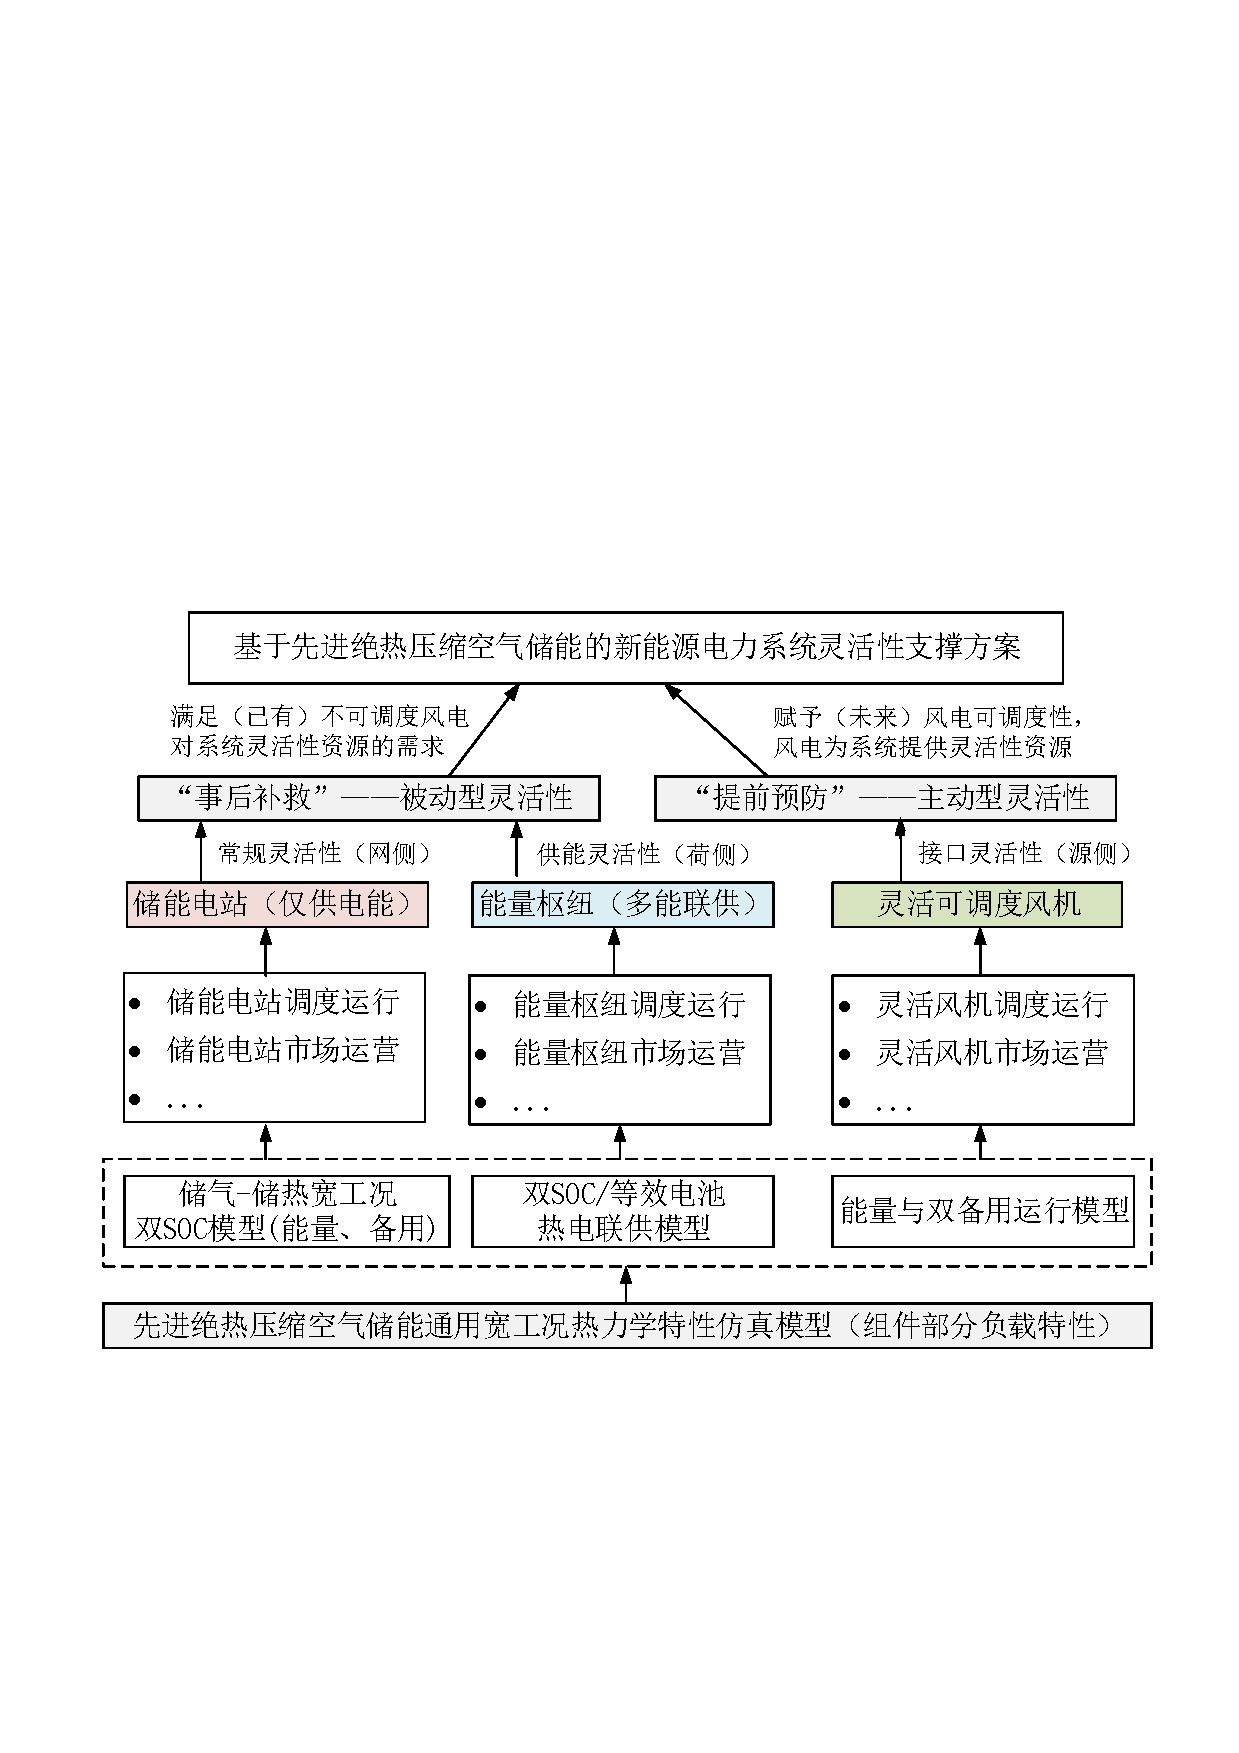
\includegraphics[scale=0.75]{figures/Chap6-Flexibility-Framework.pdf}
  \caption{基于AA-CAES的新能源电力系统灵活性支撑体系}
  \label{fig:Flexibility-Framework}
\end{figure}

%本文通过分析AA-CAES内部组件的部分负载运行特性构建了宽工况稳态热力学仿真模型,从网侧储能电站、荷侧能量枢纽、源侧灵活风机三个角度较为系统地研究了典型应用形式的设计、建模及运行与运营等问题,为充分挖掘AA-CAES这一理念的常规灵活性、供能灵活性及接口灵活性对新能源电力系统的支撑作用提供了较为系统的建模与分析方法。

总之,本文工作实现了一种“事后补救”与“提前预防”相结合的电力系统灵活性支撑方案,以网侧储能电站与荷侧能量枢纽“被动”满足当前电力系统的灵活性资源需求,提升现有电力系统对新能源的接纳能力;以源侧灵活风机在不增加(未来)风电的接入对系统灵活性资源的需求同时“主动”提供灵活性资源,从而满足未来电力系统对高比例新能源的并网消纳需求,具体如图\ref{fig:Flexibility-Framework}所示。

\section{工作展望}
\label{sec:overlook}
先进绝热压缩空气储能无疑是未来较长一段时间内机械储能领域的主要趋势,其在新能源电力系统的相关应用离不开压缩空气储能基础理论的完善。我们认为基于本文工作可进一步深入开展以下几项研究\footnote{尽管本文在撰写过程中力图避免错误,但限于对AA-CAES及其它相关领域的认知水平,文中难免存在纰漏。若您发现文中的相关错误,请通过本文的在线勘误主页(https://github.com/AIRicky/Ph.D-Thesis-On-CAES)向我们反馈。}:

\textbf{(1)构建与完善通用的先进绝热压缩空气储能仿真模型与平台,弥补国际上因压缩空气储能仿真平台不完善导致的运行研究进展缓慢的问题。}

本质上,先进绝热压缩空气储能类似于传统火电机组等,相应的仿真建模平台是深入研究其运行特性的必要前提。然而,压缩空气储能本身涉及热力学、传热学、电力学等交叉领域,导致这一仿真平台的开发难度较大,国际上相关研究进展缓慢。同时,国际上由于缺乏实际运营先进绝热压缩空气储能电站的运行数据,为该类仿真平台模型的校验等带来了不便;充分利用现有的试验型先进绝热压缩空气储能电站,积累相应的运行数据为该类仿真平台提供基础数据尤为必要。此外,本文第2章在仿真模型中并未引入压缩机、透平等各组件的控制模块,仿真功能并不完善。如何引入控制模块,扩展换热器的温度动态等,实现更短时间尺度、更精确的先进绝热压缩空气储能仿真,为AA-CAES励磁、调速等应用提供基准模型值得关注。


\textbf{(2)构建与完善兼具准确性与简单性的先进绝热压缩空气储能标准模型,为潮流计算、机组组合及经济调度等电力系统典型应用程序提供通用标准模型。}

先进绝热压缩空气储能最为典型的应用即为面向电力系统的储能电站。由于其大容量等特性,在电力系统运行框架下,先进绝热压缩空气储能需被纳入到机组组合、经济调度、实时调度及市场出清等体系,然而当前国际研究中对其模型的使用不如火电机组规范或统一。本文第3章的双SOC模型旨在实现这一目标,然而限于缺乏更详细的数据支撑,本文难以给出不同容量下典型AA-CAES储能电站部分负载运行时耗电与耗热的标准特性曲线,双SOC模型的应用范围或应用条件等尚需进一步深入研究。


\textbf{(3)构建与完善先进绝热压缩空气储能的热电多能联供运行域,及系统化的多能联供建模方法,为热电联合调度提供标准化模型。}

不同于其它类型的储能,先进绝热压缩空气储能具有多能联供特性,其可等效视为热电联产机组与储电及储热单元的组合体。在热电调度中,热电联产机组存在标准化的凝汽式与背压式的热电凸形或非凸形可行域模型,然而压缩空气储能由于其热电联供模式的灵活性,其供热功率既可来自存储的压缩热、透平乏气,又可来自辅助的外部热源等,目前缺乏统一的热电可行域标准。本文第4章将现有研究中普遍存在的压缩空气储能型多能联供系统抽象为两类并给出了相应的热电联供模型,但是未给出在各种热源条件下的热电运行可行域,也未形成相应的标准化可行域。在后续研究中应构建类似于热电联产机组的压缩空气储能热电联供可行域及相应的凸化方法,并在可行域中引入储电与储热赋予的多时段耦合信息,为国际上基于压缩空气储能的多能联供提供标准的模型。


\textbf{(4)构建与完善系统化的内嵌先进绝热压缩空气储能的灵活可调度风机设计体系,并基于试验数据验证灵活风机的修正风功率曲线。}

在电源侧风电与压缩空气储能集成领域,目前已存在多种类型的风-储集成设计方法,各类方法均有适应的场景。本文第5章的灵活风机对永磁直驱风机的适应性更强一些,如何针对双馈型风机设计该类内嵌压缩空气的灵活性方案,以及如何针对典型的应用场景实现内部各组件的系统化的容量配置方案,进而实现灵活风机性能的优化值得深入研究。此外,本文研究中并未仔细衡量价格预测误差等对灵活风机经济性的影响,事实上,价格预测误差将会使得灵活风机的收益受损,灵活风机利用其双备用特性,继续参与备用市场带来的额外收益是否能实现与价格误差导致的收益折损之间的平衡,值得结合大量备用市场数据深入研究。
